%TODO Done

\section{Canonical Finite State Machine Example}

Grammar:\\
$S \rightarrow A\$$\\
$A \rightarrow aCD$\\
$A \rightarrow ab$\\
$C \rightarrow c$\\
$D \rightarrow d$\\

CFSM:\\
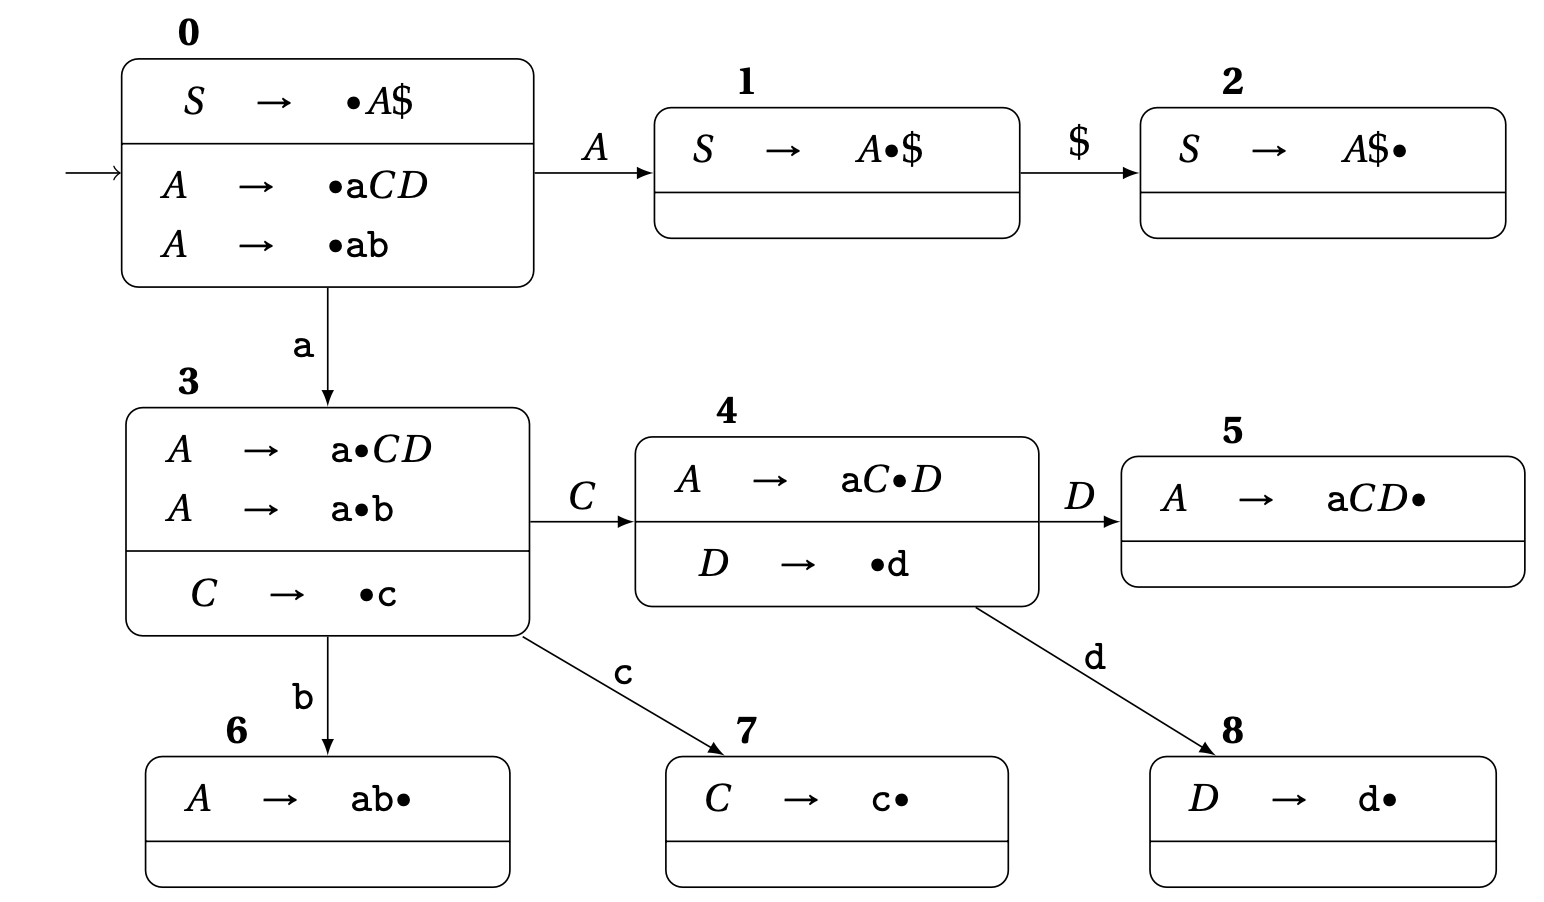
\includegraphics[height=5cm]{../images/Pasted image 20250317175419.png}

The language of this grammar is LR(1).


% Adding a concise step-by-step guide for building the CFSM
\section*{Steps to Construct the Canonical Finite State Machine (CFSM)}
\begin{enumerate}
    \item \textbf{Augment the Grammar}: Add a new start symbol \( S' \) and production \( S' \to S \$ \), where \( S \) is the original start symbol and \( \$ \) is the end-of-input marker.
    \item \textbf{Initialize the First State}: Compute the initial state \( I_0 = \text{CLOSURE}(\{[S' \to \cdot S \$]\}) \), where the dot (\(\cdot\)) indicates the current position in the production.
    \item \textbf{Compute CLOSURE}: For a set of items \( I \):
        \begin{itemize}
            \item Start with \( \text{CLOSURE}(I) = I \).
            \item For each item \( [A \to \alpha \cdot B \beta, w] \) in \( \text{CLOSURE}(I) \), where \( B \) is a nonterminal:
                \begin{itemize}
                    \item For each production \( B \to \gamma \), compute \( \text{FIRST}_1(\beta w) \).
                    \item For each \( u \in \text{FIRST}_1(\beta w) \), add \( [B \to \cdot \gamma, u] \) to \( \text{CLOSURE}(I) \) if not present.
                \end{itemize}
            \item Repeat until no new items are added.
        \end{itemize}
    \item \textbf{Compute GOTO}: For a state \( I \) and symbol \( X \) (terminal or nonterminal):
        \begin{itemize}
            \item Initialize \( J = \emptyset \).
            \item For each item \( [A \to \alpha \cdot X \beta, w] \) in \( I \), add \( [A \to \alpha X \cdot \beta, w] \) to \( J \).
            \item Return \( \text{CLOSURE}(J) \).
        \end{itemize}
    \item \textbf{Build the State Machine}:
        \begin{itemize}
            \item Initialize the set of states \( C = \{I_0\} \) and worklist \( W = \{I_0\} \).
            \item While \( W \neq \emptyset \):
                \begin{itemize}
                    \item Remove a state \( I \) from \( W \).
                    \item For each symbol \( X \) where \( \text{GOTO}(I, X) \neq \emptyset \):
                        \begin{itemize}
                            \item Let \( J = \text{GOTO}(I, X) \).
                            \item If \( J \notin C \), add \( J \) to \( C \) and \( W \).
                            \item Add transition \( I \xrightarrow{X} J \) to the automaton.
                        \end{itemize}
                \end{itemize}
        \end{itemize}
    \item \textbf{Construct the Parsing Table}:
        \begin{itemize}
            \item For each state \( I \in C \):
                \begin{itemize}
                    \item If \( [A \to \alpha \cdot a \beta, w] \in I \) and \( \text{GOTO}(I, a) = J \), add shift action to state \( J \) for terminal \( a \).
                    \item If \( [A \to \alpha \cdot, w] \in I \), add reduce action by \( A \to \alpha \) for lookahead \( w \).
                    \item If \( [S' \to S \cdot \$] \in I \), add accept action for \( \$ \).
                \end{itemize}
            \item Check for conflicts: Shift-reduce or reduce-reduce conflicts indicate the grammar is not LR(1).
        \end{itemize}
\end{enumerate}
